\chapter{Integração do AppMan com a especificação {DRMAA}}
\label{cap:implementacao}

O protótipo AppMan ainda está em desenvolvimento, portanto nem todos os requisitos descritos no modelo GRAND constam no protótipo e, seu funcionamento ainda apresenta alguns comportamentos inesperados. 

Desenvolvido em grupo com seu código fonte aberto, seus fontes estão acessíveis para qualquer um que deseja visualizá-los. 

Em um primeiro momento foi feita uma análise das versões existentes no repositório com controle de versões gerenciado pelo \emph{software Subversion}. Dentre as versões analisadas foi encontrado em uma ramificação (\emph{branch}) deste repositório uma versão do AppMan que constava uma implementação da integração, teoricamente, realizada e funcional com o uso da DRMAA. Ao efetuar testes com esta versão foi constatado que não estava funcional. Alguns ajustes, que serão explicados posteriormente, foram necessários para o funcionamento correto desta versão.

\section{Criação do Ambiente Computacional}

Para o desenvolvimento do trabalho foi necessário a configuração de um servidor LDAP (APENDICE A) pré-requisito para a execução do \emph{middleware} EXEHDA/ISAM onde é executado o AppMan. Alguns problemas foram encontrados na configuração deste servidor. Um dos motivos foi o fato da documentação existente para a instalação e configuração do protótipo estar desatualizada com as versões do LDAP e distribuições do sistema operacional Linux existente atualmente. 

Também foi criado um ambiente computacional com um RMS PBS instalado possuindo três nós para submissão e execução de tarefas. A instalação do OpenPBS (APENDICE B) foi feita em um computador com processador AMD Turion(tm) 64 X2 Mobile Technology TL-50 1.6Ghz e 1.5Gb de memória RAM. Nesta configuração/instalação do PBS foi usado um passo à passo, porém foi necessário a alteração nos parâmetros de configuração (\textbf{--with-scp}) para a compilação do RMS. Essa alteração faz com que o PBS deixe de fazer o \emph{stage-in/stage-out} com o comando padrão \textbf{pbs\underline{ }rcp} para usar o comando \textbf{scp} que é o comando padrão para cópia segura dos sistemas operacionais Linux.

O Servidor LDAP foi instalado em um computador AMD Athlon(tm) 64 X2 Dual Core Processor 4000+ 2.2Ghz e memória RAM de 2.0Gb. Este computador também está na lista de nós do PBS além de mais dois outros. O primeiro possui processador AMD Sempron(tm) 2500+ 1.8Ghz e memória RAM de 512Mb e o outro possui um processador Intel(R) Celeron(R) 2.00GHz com 512Mb de memória RAM. Em todos os computadores o sistema operacional é Linux Ubuntu 7.10 com Kernel 2.6.22.

Outro pré-requisito para o funcionamento do protótipo é a instalação do servidor \emph{Network File System} (NFS), usado para compartilhamento de arquivos no Linux. A versão atual do protótipo necessita que o diretório onde as tarefas são criadas seja compartilhado. Esta é uma necessidade que não faz parte do modelo GRAND.

Para compilação e alterações nos fontes do protótipo foi usado as IDEs NetBeans\cite{netbeans} e Eclipse\cite{eclipse}, para geração de diagramas UML bem como a engenharia reversa do AppMan, foi usado, além das IDEs citadas, o software Umbrello\cite{umbrello}.

\section{Componente DRMAA (submissão e monitoração)}

Baseado na implementação desenvolveu-se um modelo definido por um conjunto de classes conforme Figura~\ref{fig:UML_DRMAA}. Os principais métodos necessários para submissão e monitoração de uma tarefa estão na classe \emph{appman.rmswrapper.pbs.drmaa.SessionImpl} que implementa a \emph{interface} \emph{org.ggf.drmaa.Session}.

A DRMAA java \emph{binding} foi implementada com a JAVA \emph{Native Interface} (JNI). JNI é uma \emph{interface} de padrão de programação para escrever métodos Java sob uma máquina virtual Java (JVM), fazendo chamadas recebendo chamadas de aplicações nativas. Essas aplicações nativas, são aplicações específicas do sistema operacional. Dentre as linguagens, pode-se fazer chamadas em C++, C e \emph{Assembly} \cite{jni}.

Dentre os inúmeros métodos existentes na classe \emph{SessionImpl} os mais relevantes para o AppMan são:

\begin{itemize}
	\item \emph{String runJob(JobTemplate jobTemplate)} submete uma tarefa e tem como retorno um identificador para ser usado se necessário.
	\item \emph{JobInfo wait(String jobName, long timeout)} espera o final da execução por um determinado tempo máximo.
	\item \emph{appman.rmswrapper.pbs.drmaa.JobTemplateImpl} encapsula a definição de uma tarefa para submissão.
	\item \emph{appman.rmswrapper.pbs.drmaa.JobInfoImp} representa a tarefa após a sua execução.
\end{itemize}

A implementação de DRMAA usada foi a mesma usada na implementação com o GridWay 1.0 \cite{Herrera2007} sendo implementada apenas as \emph{interfaces} essenciais para a submissão das tarefas. 

\begin{figure}[htb]
\begin{center}
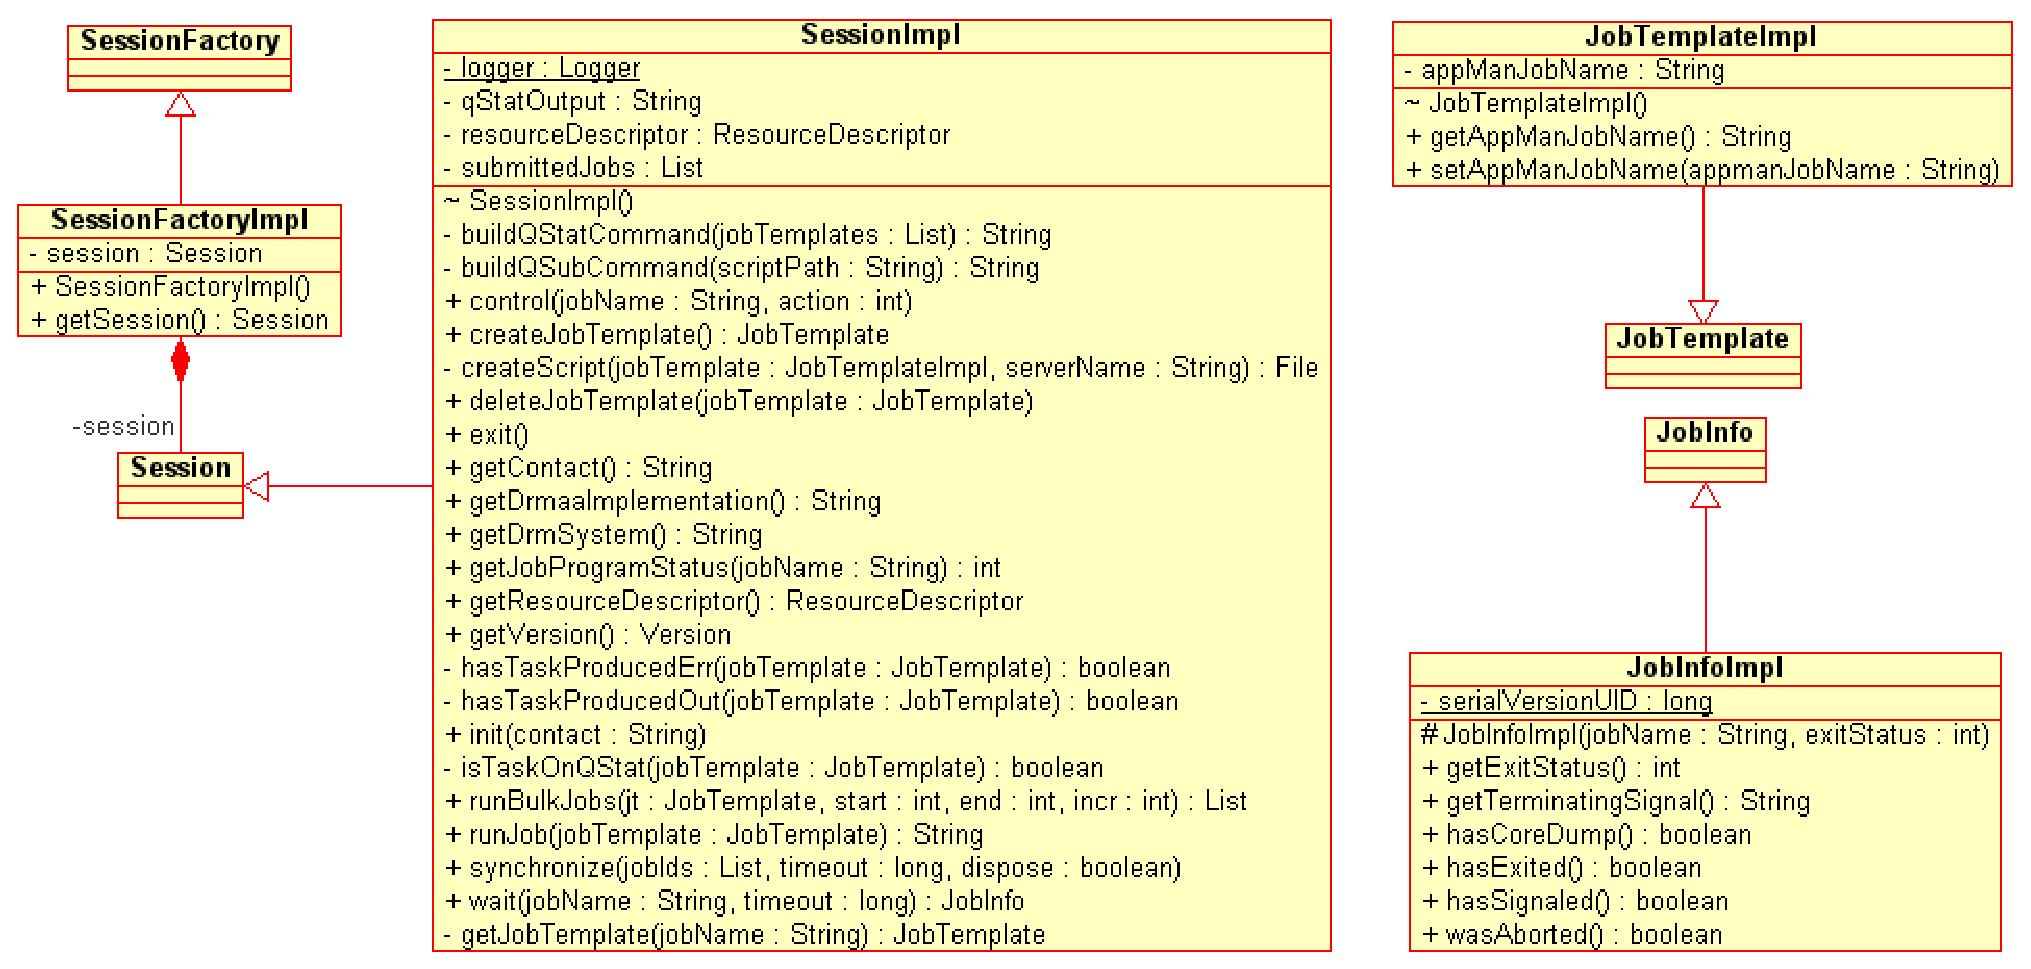
\includegraphics[scale=0.5]{./img/drmaaUML2.eps}
\caption{Diagrama de classes do pacote \textbf{appman.rmswrapper.pbs.drmaa}}
\label{fig:UML_DRMAA}
Fonte: Autoria Própria
\end{center}
\end{figure}

Apesar de, não tão relevante quanto os métodos citados acima, o método \emph{createScript} sofreu uma pequena modificação. Este método retorna um arquivo (\emph{File}) que é o \emph{script} que será submetido para o PBS. Neste método foi feito uma alteração na geração do \emph{script} (ANEXO A) que é submetido ao PBS. Em sua forma inicial, notou-se que as tarefas estavam sendo submetidas para o nó padrão de submissão do PBS. Para que as tarefas fossem distribuídas de forma pseudo-randômica entre os nós disponíveis adicionou-se a seguinte linha no arquivo de submissão:

\textbf{\#PBS -l nodes=x}

Onde \textbf{x} é um número gerado pseudo-aleatóriamente entre 1 e 3 que são os nós disponíveis.

\section{AppMan com DRMAA}

Conforme análise do código encontrado no repositório, a integração ficou concentrada em duas mudanças. A primeira é a criação de uma classe nova \emph{appman.GridTaskDrmaa} e a outra foi uma alteração no arquivo de configuração que indica em qual componente é responsável para execução da tarefa, ou \emph{middleware} EXEHDA, ou nova implementação. Com isso, o impacto da modificação torna-se relativamente baixo. 

\subsection{Classe GridTaskDrmaa}

A nova classe implementa a mesma \emph{interface} que a classe padrão \emph{appman.GridTask}. A maior alteração encontra-se no método \emph{execute} onde são feitas as chamadas ao componente de submissão. O método \emph{execute} Figura~\ref{fig:execute}, é onde são realizados os passos indicados pela especificação DRMAA na submissão e monitoração de tarefas.

\begin{figure}[htb]
\begin{center}
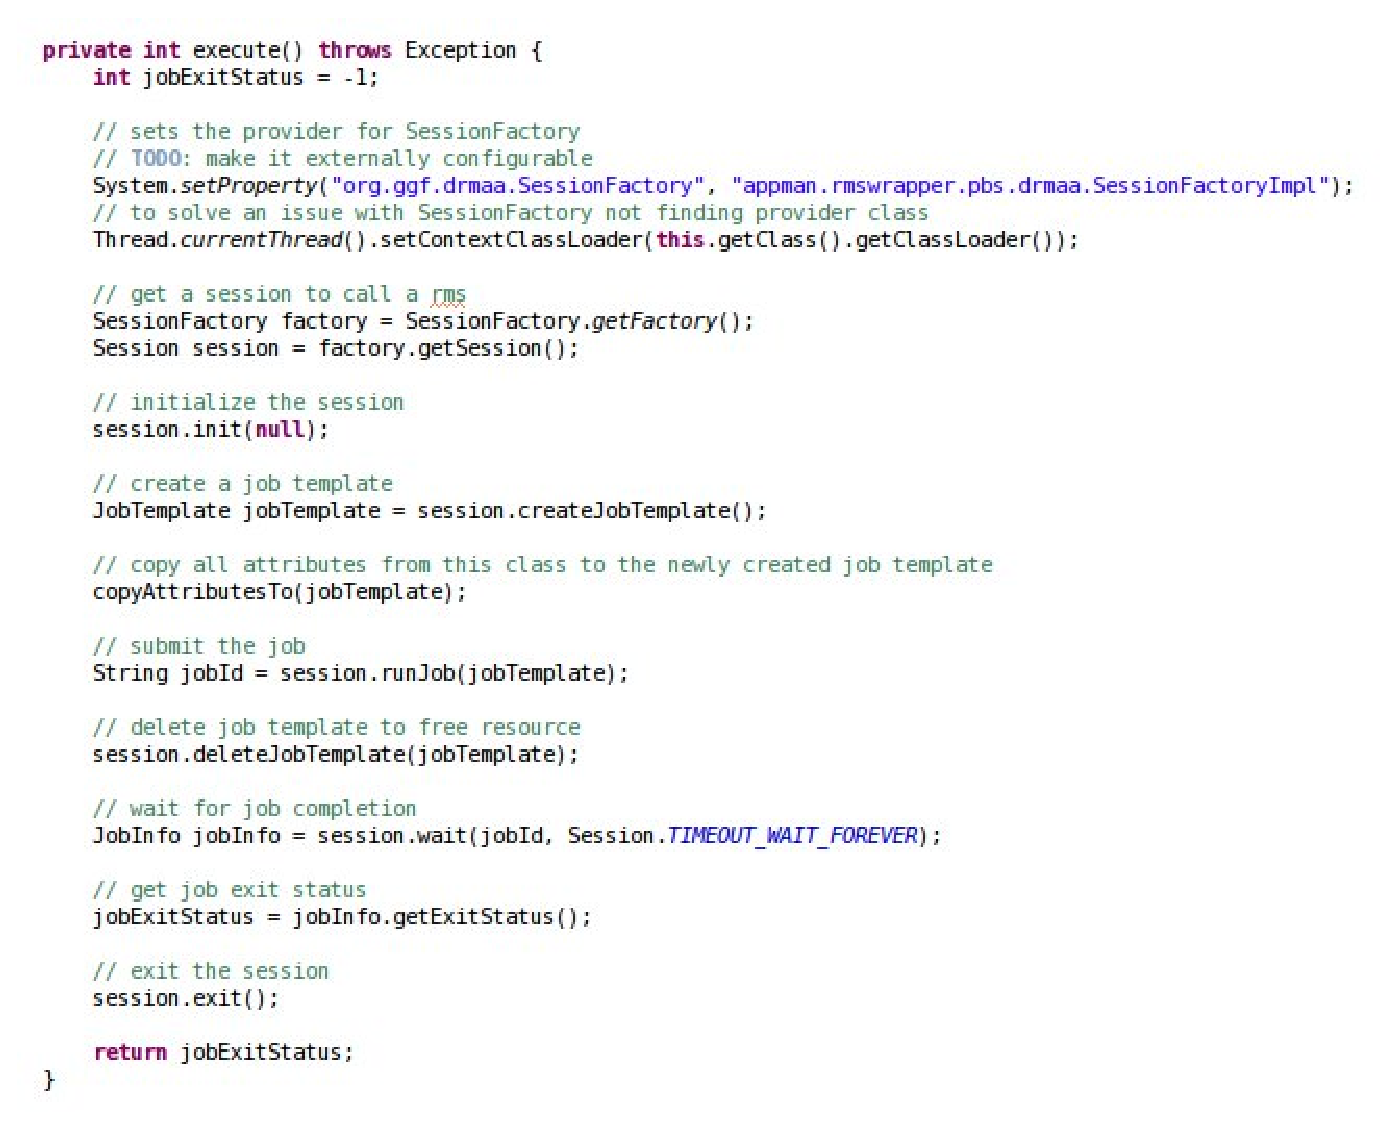
\includegraphics[scale=0.65]{./img/execute.eps}
\caption{Método \emph{execute} da nova classe \emph{appman.GridTaskDrmaa}}
\label{fig:execute}
Fonte: Autoria Própria
\end{center}
\end{figure}

\subsection{Arquivo de configuração}

A alteração no arquivo de configuração foi feita para que o nó saiba que componente usar na submissão da tarefa. Esta alteração consiste na criação de uma propriedade que recebe o valor que indica qual componente usar. A figura x exemplifica o arquivo de configuração onde o \emph{Submission Manager} criado no nó \textbf{0.desktop} usará a \emph{GridTaskDrmaa} para submeter tarefas e o nó \textbf{0.notebook} usará \emph{GridTask} para submeter.

\begin{figure}[htb]
\begin{center}
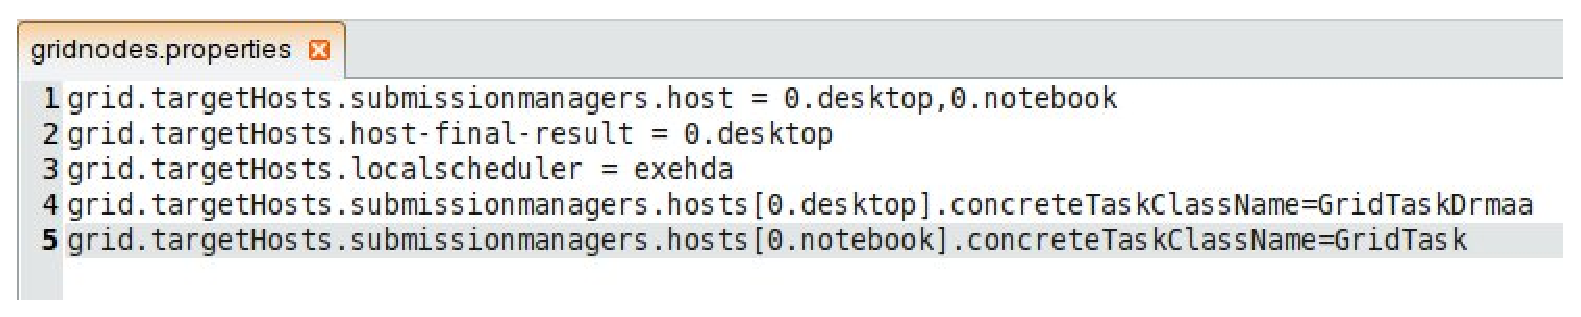
\includegraphics[scale=0.5]{./img/gridnodes_properties.eps}
\caption{Arquivo de configuração \emph{gridnodes.properties}}
\label{fig:gridonodes_properties}
Fonte: Autoria Própria
\end{center}
\end{figure}

Para que esta nova configuração fosse reconhecida foi criado o método \emph{loadConcreteTaskClassName} na classe \emph{TaskManager} conforme mostra a figura~\ref{fig:Concrete} o qual lê a propriedade no arquivo de configuração e retorna o nome do componente configurado para onde submeter a tarefa. Na implementação atual não foi possível, conforme sugerido, a criação de um \emph{Submission Manager} que submete tarefas via componente DRMAA e um \emph{Submission Manager} usando o componente padrão ao mesmo tempo.

\begin{figure}[htb]
\begin{center}
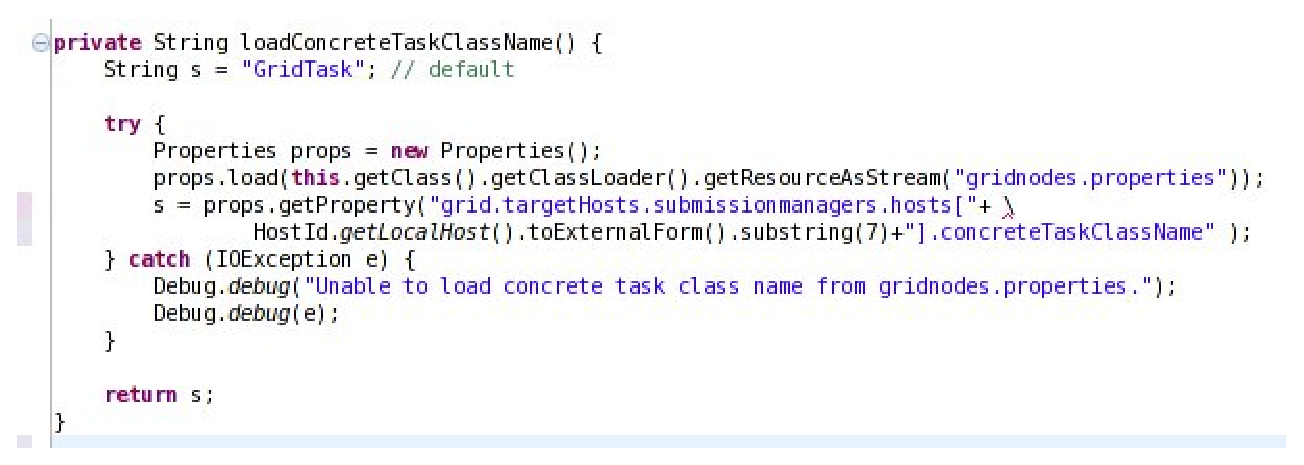
\includegraphics[scale=0.7]{./img/concrete.eps}
\caption{Método \emph{loadConcreteTaskClassName}}
\label{fig:Concrete}
Fonte: Autoria Própria
\end{center}
\end{figure}